\documentclass{article}
\usepackage{amsmath,amsthm,amssymb}
\usepackage{mathtext}
\usepackage[T2A]{fontenc}
\usepackage[utf8]{inputenc}
\usepackage[english]{babel}
\usepackage{graphicx}
\usepackage{hyperref}
\usepackage{longtable}
\usepackage{booktabs}
\usepackage{multirow}

\title{Domain adaptation of transformers model for products search}
\author{Algis Dumbris}
\date{December 2020}



\begin{document}
\maketitle
\begin{abstract}
    The project report contains a description of experiments for domain adaptation of transformers model for products search. Project code: \url{https://github.com/Dumbris/semantic-search-domain-adaptation}, Dataset \url{https://www.kaggle.com/c/home-depot-product-search-relevance/data}.
\end{abstract}



\section{Introduction}
	Using transformer models (BERT, RoBERTa, GPT) over the last two years demonstrates significant quality improvements on many NLP tasks. 
	For many companies selling products on the Internet, the search function is a core function. For such companies, search relevancy is a measure of how quickly they can get customers to the right products. 
	
	Traditionally for product search uses term-matching algorithms (BM25) builtin into ElasticSearch or Solr. But these systems may fail when queries and product descriptions use different terms to describe the same meaning. Semantic search based on transformer models could help in this case.
In my research, I am trying to find the best methods for the domain adaptation of transformer models for improving search relevancy. I intentionally avoid any data preprocessing here and try to use text data as is for transformers models. 
\subsection{Team}
The author of this project is \textbf{Algis Dumbris}.



\section{Related Work}
\label{sec:related}

The paper \cite{reimers-2019-sentence-bert} describes how Sentence Embeddings implemented and how it can be used in search and ranking tasks.

\cite{padigela2019investigating} - Comparation BERT and BM25 algorithm performance on MS MARCO dataset.

\section{Dataset Description}

I am using the Home Depot Product Search Relevance dataset from Kaggle. The dataset contains real customer search terms from Home Depot's website. In total dataset contains 186135 pairs of query and product with relevancy label.  
	Home Depot has crowdsourced the search/product pairs to multiple human raters to create the ground truth labels. The relevance label is a number between 1 (not relevant) to 3 (highly relevant). For example, a search for "AA battery" would be considered highly relevant to a pack of size AA batteries (relevance = 3), mildly relevant to a cordless drill battery (relevance = 2), and not relevant to a snow shovel (relevance = 1).

\begin{table}[tbh!]
\begin{center}
\begin{tabular}[t]{|l|ccc|}
\hline
%\cline{2-4}
Type & Train & Test & \\
\hline
Queries & 19384  & 4845  & \\
Docs & 149143 & 36992 & \\
Added With Negative Samples & 298270 & & \\
\hline
\end{tabular}
\caption{Statistics of the Train / Test split}
\label{tab:statistics}
\end{center}
\end{table}

\begin{table}[tbh!]
\centering
\caption{Samples of query / docs / relevancy data}
\begin{tabular}{llr}
\toprule
  query &                                      product\_title &  relevance \\
\midrule
 \multirow{7}{*}{zwave switch} &  GE Z-Wave 1800-Watt Resistive CFL-LED Indoor P... &        3.0 \\
 &  Leviton Z-Wave Controls 3-Way/Remote Scene Cap... &        3.0 \\
 &  Leviton Decora Z-Wave Controls 15 Amp Scene Ca... &        3.0 \\
 &  GE Home Automation 120 VAC 3-Way Auxiliary Add... &        3.0 \\
 &  GE Z-Wave 600 Watt CFL-LED Indoor In-Wall Dimm... &        2.7 \\
 &  Z-Wave Wireless Lighting Control with Keypad C... &        2.7 \\
 &  Lutron Aurora Wireless Lighting Control System... &        2.3 \\
 &  Leviton Z-Wave Enabled 15 Amp Scene Capable Re... &        2.0 \\
 \hline
 \multirow{7}{*}{\$ hole saw} &            Milwaukee Metal Hole Saw Kit (15-Piece) &        3.0 \\
 &                  Milwaukee 4 in. Bi-Metal Hole Saw &        3.0 \\
 &        Milwaukee 6-3/8 in. Recessed Light Hole Saw &        3.0 \\
 &         PRO-SERIES 19-Piece Hole Saw Set with Case &        2.3 \\
 &                       Ryobi Hole Saw Set (6-Piece) &        2.3 \\
 &          Bosch Daredevil Spade Bit Set (10-Pieces) &        2.0 \\
 &      Milwaukee 3/8 in. Ergo Quick-Change Saw Arbor &        2.0 \\
 &  Milwaukee 2 in. to 7 in. Dia. Adjustable Hole ... &        1.3 \\
\bottomrule
\end{tabular}
\end{table}

	In my experiments, for matching, I am using only the product name text attribute. The product description text attribute potentially useful for pretraining using a masked language modeling task (MLM). It's left for future experiments.

\section{Experiment Description}
I wrote a python library that allows to change experiment parameters, manipulate datasets, and calculate metrics for conducting experiments. The general scheme of experiments is presented on Fig.~\ref{fig:experiment}. 
In the beginning, the whole dataset split on the train and test parts. While the model is trained, on some steps, the evaluator starts metrics calculation on test data. 
On the test step, the evaluator rebuilds the docs candidates list for each query using the trained model. These candidates list compared with the real docs list for metrics calculation. 

\begin{figure}[!tbh]
    \centering
    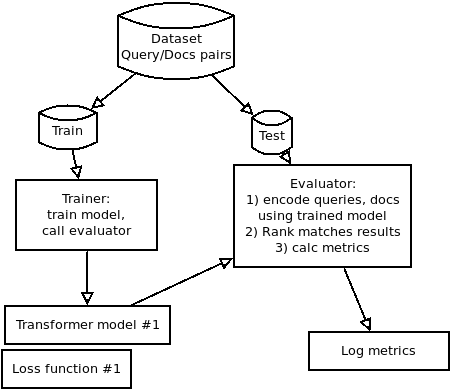
\includegraphics[width=1\linewidth]{Experiment_diagram.png}
    \caption{Experiment design.}
    \label{fig:experiment}
\end{figure}

In current setup I am using losses: $CosineSimilarityLoss$ - The similarity of these embeddings is computed using cosine similarity and the result is compared to the gold similarity score.
$SoftmaxLoss$ - adds a softmax classifier on top of the output of two transformer networks.
I am using three pretrained models from package sentence\_transformers msmarco-distilroberta-base-v2,  distilbert-base-nli-stsb-quora-ranking, LaBSE.

\subsection{Metrics} 
I am using Normalized Discounted Cumulative Gain (nDCG@k) @3, @10. And Mean average precision (MAP@k) @3, @10


\subsection{Results}

Results for best-trained models are presented in Table.~\ref{tab:results_ndcg} for comparison, I have added BM25 and Universal Sentence Encoder models.
On nDCG@10, metrics transformers give results slightly worse than the BM25 algorithm. On Map@k metrics, transformers showed poor performance - BM25 Map@3 is 0.27, but the best transformer model gives only 0.012.

\begin{table}[hbt!]
\centering
\caption{nDCG metrics on the test dataset, after training.}
\begin{tabular}{llrr}
\toprule
                             model &         loss &  \textbf{nDCG@10} &  nDCG@3 \\
\midrule

                                   BM25 &                       &           0.3908 &          0.3450 \\
            \textbf{sentence-transformers/LaBSE} &  \textbf{CosineSimilarityLoss} &           \textbf{0.3708} &          0.3408 \\
 distilbert-base-nli-stsb-quora-ranking &  CosineSimilarityLoss &           0.3564 &          0.3238 \\
            sentence-transformers/LaBSE &           SoftmaxLoss &           0.3478 &          0.3136 \\
          distilroberta-base-msmarco-v2 &  CosineSimilarityLoss &           0.2934 &          0.2608 \\
 distilbert-base-nli-stsb-quora-ranking &           SoftmaxLoss &           0.2846 &          0.2487 \\
          distilroberta-base-msmarco-v2 &           SoftmaxLoss &           0.2635 &          0.2301 \\
           universal-sentence-encoder/4 &                       &           0.2326 &          0.1867 \\           
           
\bottomrule           
\label{tab:results_ndcg}
\end{tabular}
\end{table}


\begin{table}[hbt!]
\centering
\caption{MAP metrics on the test dataset, after training.}
\begin{tabular}{llrr}
\toprule
                             model &         loss &  \textbf{MAP@10} &  MAP@3 \\
\midrule

                                   BM25 &                       &          0.2375 &         0.2754 \\
           universal-sentence-encoder/4 &                       &          0.0091 &         0.0138 \\
            \textbf{sentence-transformers/LaBSE} &           \textbf{SoftmaxLoss} &          \textbf{0.0080} &         0.0124 \\
 distilbert-base-nli-stsb-quora-ranking &           SoftmaxLoss &          0.0080 &         0.0120 \\
          distilroberta-base-msmarco-v2 &  CosineSimilarityLoss &          0.0078 &         0.0119 \\
            sentence-transformers/LaBSE &  CosineSimilarityLoss &          0.0077 &         0.0112 \\
 distilbert-base-nli-stsb-quora-ranking &  CosineSimilarityLoss &          0.0076 &         0.0112 \\
          distilroberta-base-msmarco-v2 &           SoftmaxLoss &          0.0076 &         0.0110 \\
           
\bottomrule           
\label{tab:results_map}
\end{tabular}
\end{table}

To understand how metrics on test data are changing during training, you can check Fig.~\ref{fig:ndcg10}. One epoch on these graphs contains 7000 steps. You can see that after the first epoch, metrics almost don't change.

\begin{figure}[hbt!]
    \centering
    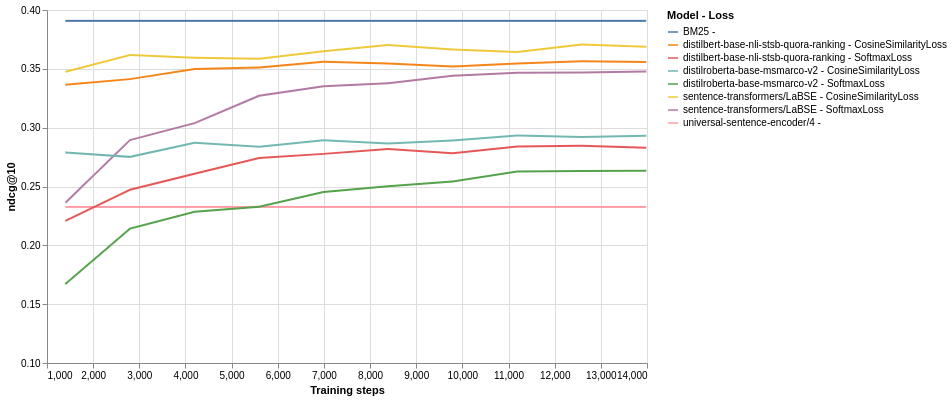
\includegraphics[width=1\linewidth]{visualization_ndcg10.png}
    \caption{nDCG@10 metrics.}
    \label{fig:ndcg10}
\end{figure}

\begin{figure}[!tbh]
    \centering
    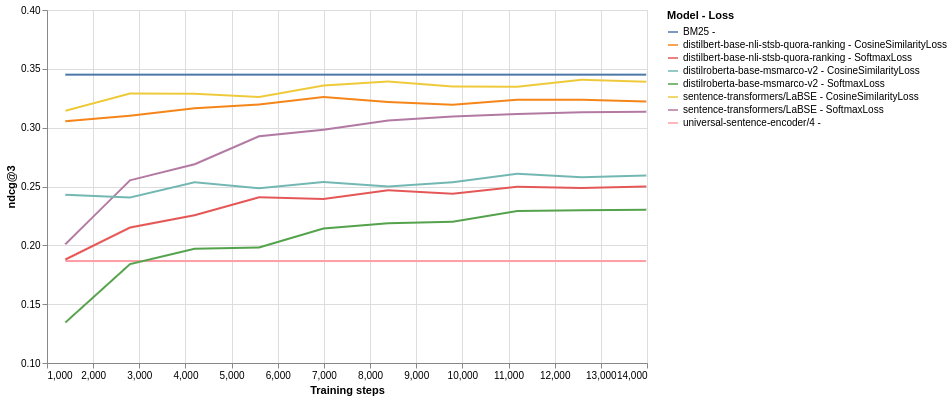
\includegraphics[width=1\linewidth]{visualization_ndcg3.png}
    \caption{nDCG@3 metrics.}
    \label{fig:ndcg3}
\end{figure}

\begin{figure}[!tbh]
    \centering
    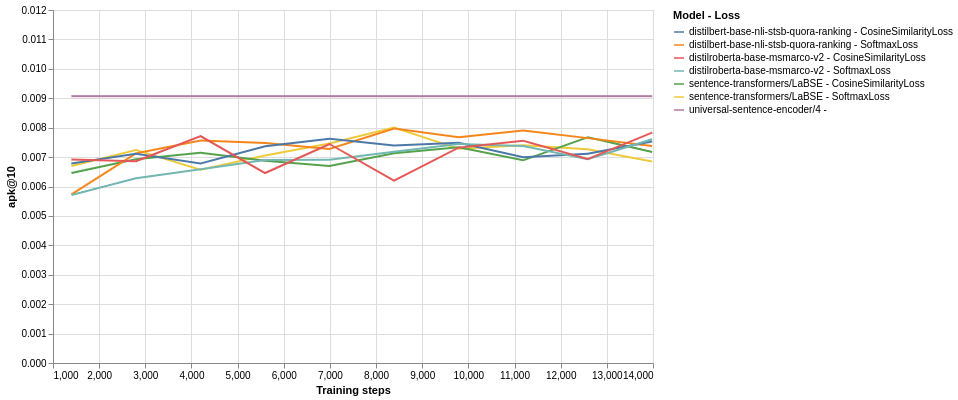
\includegraphics[width=1\linewidth]{visualization_apk10.png}
    \caption{MAP@10 metrics.}
    \label{fig:apk10}
\end{figure}

\begin{figure}[!tbh]
    \centering
    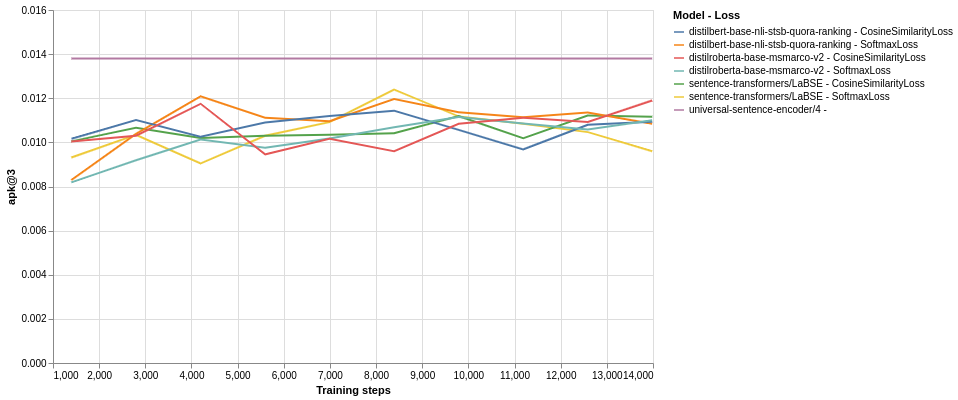
\includegraphics[width=1\linewidth]{visualization_apk3.png}
    \caption{MAP@3 metrics.}
    \label{fig:apk3}
\end{figure}

\clearpage

\section{Conclusion}
I tried to apply BERT and RoBERTa models for product search using the product title in this project. On the current dataset, using just fine-tuning on annotated data, transformers models give results worse than the BM25 algorithm. I think it is related to the nature of data. Product names contain plenty of abbreviations, numbers, etc. Also, query and product titles are usually short and do not allow to leverage context information. 
Between distilled models: better performance showed by models were first trained on NLI data, then fine-tuned on the STS benchmark dataset,  and finally fine-tuned on the annotated domain-specific dataset using cosine similarity loss. 

\bibliographystyle{apalike}
\bibliography{lit}
\end{document}
